\documentclass[]{article}
\setlength{\marginparwidth}{0.5in}
\usepackage{amsmath,amssymb,amsthm,mathtools,booktabs}
\usepackage{alltt,xspace,array,tikz,pifont,comment,graphicx}
\usepackage[author-year]{amsrefs}
\input FJHDef.tex

\providecommand{\HickernellFJ}{Hickernell}
\DeclareMathOperator{\integ}{\texttt{\textup{integral}}}
\DeclareMathOperator{\goodinteg}{\texttt{\textup{int}}}
\DeclareMathOperator{\flawinteg}{\texttt{\textup{flawint}}}
\DeclareMathOperator{\ballinteg}{\texttt{\textup{ballint}}}
\DeclareMathOperator{\Var}{Var}
\newcommand{\tVar}{\widetilde{\Var}}
\DeclareMathOperator{\err}{err}
\DeclareMathOperator{\size}{size}
\DeclareMathOperator{\maxcost}{maxcost}
\DeclareMathOperator{\mincost}{mincost}
\newcommand{\oerr}{\overline{\err}}
\newcommand{\herr}{\widehat{\err}}
\newcommand{\terr}{\widetilde{\err}}

\newtheorem{theorem}{Theorem}
\newtheorem{prop}[theorem]{Proposition}
\newtheorem{lem}{Lemma}
\newtheorem{cor}{Corollary}
\theoremstyle{definition}
\newtheorem{algo}{Algorithm}
\newtheorem*{ballalgo}{Algorithm $\ballinteg$}
\newtheorem*{flawalgo}{Algorithm $\flawinteg$}
\newtheorem{condit}{Condition}
%\newtheorem{assump}{Assumption}
\theoremstyle{remark}
\newtheorem{rem}{Remark}
\newcommand{\Fnorm}[1]{\abs{#1}_{\cf}}
\newcommand{\Gnorm}[1]{\abs{#1}_{\cg}}
\newcommand{\flin}{f_{\text{\rm{lin}}}}
\DeclareMathOperator{\INT}{INT}
\DeclareMathOperator{\tri}{peak}
\DeclareMathOperator{\twopk}{twopk}
\newcommand{\datasites}{\{x_i\}_{i=0}^n}

\begin{document}

\title{Reliable Adaptive Numerical Integration for Cones of Integrands}
\author{Fred J. Hickernell, Martha Razo, and Sunny Yun}
\maketitle 


\begin{abstract} Hi this is the abstract
\end{abstract}

\section{Introduction} 

While some mathematical problems can be solved using pencil and paper, many others must be solved by numerical algorithms.  Software libraries such as the NAG library \cite{NAG23} and languages for numerical computation, such as MATLAB \cite{MAT8.3}, Mathematica, \cite{Mat9a} and R \cite{R3.03_2013}, are able to solve a wide variety of mathematical and statistical problems.  Many of the numerical algorithms in these software packages are \emph{adaptive}, meaning that they automatically expend the right amount of computational effort needed to (hopefully) provide an approximate solution with an error no greater than the tolerance. MATLAB's \texttt{integral} for integration, \texttt{fminbnd} for optimization, and \texttt{ode45} for solving ordinary differential equations are examples of adaptive algorithms.  The Chebfun MATLAB toolbox \cite{TrefEtal14} is a whole suite of adaptive algorithms.  

At the core of every adaptive algorithm is a method for estimating the error of the numerical approximation based on the computations already performed.  Unfortunately, these error estimates either require too much information from the user or are typically based on heuristics and not guaranteed. Our aim is to rectify this deficiency---starting with the problem of numerical integration (quadrature).

Various analytic methods for evaluating integrals are taught in calculus courses, e.g., substitution, integration by parts, and partial fractions.  Unfortunately, the antiderivatives of many elementary functions \emph{cannot} be expressed as elementary functions, no matter how clever one is.  One important example arising in statistical inference is the standard normal probability density, $\phi: x \mapsto \me^{-x^2/2}/\sqrt{2 \pi}$, whose integral is the standard normal cumulative distribution, $\Phi : x \mapsto \int_{-\infty}^x \phi(t) \, \dif t$.  Since the $\Phi$ is not an elementary function, values of $\Phi$ must be provided via tables in statistics textbooks and special functions in calculators. By contrast, the derivatives of elementary functions are always elementary functions.  

We want an algorithm $\integ$, that is \emph{guaranteed} to provide a numerical approximation to the true integral with an error no greater than a specified error tolerance, namely,
\begin{equation*}
\abs{\int_a^b f(x) \, \dif x - \integ(f,a,b,\varepsilon)} \le \varepsilon \qquad \forall f \in \cc,\ a, b \in \reals, \ a < b, \ \varepsilon > 0,
\end{equation*}
where $a$ and $b$ are finite with $a<b$, and $\cc$ is some clearly defined set of integrands.  The input $f$ is a black-box algorithm that produces $f(x)$ for any given $x \in [a,b]$.  The definition of $\cc$ will entail some general assumptions about $f$, but the user should not be required provide more detailed information about $f$.

Here we discuss \emph{three} automatic numerical integration algorithms based on the trapezoidal rule, 
\begin{multline} \label{trapruledef}
T_n(f) := \frac{b-a}{2n} [ f(t_0) + 2 f(t_1) + \cdots  + 2 f(t_{n-1}) + f(t_n)], \\
t_i=a+\frac{i(b-a)}{n}, \ i=0, \ldots, n, \ n \in \naturals := \{1, 2, \ldots \},
\end{multline}
whose fundamental properties are reviewed in Sect.\ \ref{trapbasicsec}.  The first two algorithms are well-known, while the third is new.  Each algorithm takes a different approach to the problem of choosing the number of trapezoids required to meet the error tolerance.
\begin{itemize}
\item Students often see the trapezoidal rule in their calculus course, where they learn the formula, \eqref{trapruledef}, and are provided an error bound, such as \eqref{traperrbd}.  Students might use the non-adaptive algorithm $\ballinteg$ presented in Sect.\ \ref{autoballsec}.  This algorithm requires an upper bound on the variation of $f'$.  If the user chooses a modest upper bound, then $\ballinteg$ will work fine for integrands such as $f_{\text{easy}}$, defined below in \eqref{feasy}, but $\ballinteg$ will fail for integrands like the others plotted in Fig.\ \ref{fourintegfig}, whose first derivatives with large variations.

\item Courses in numerical analysis teach students to estimate the absolute error of $T_n(f)$ by $\abs{T_n(f)-T_{n/2}(f)}/3$.  This error estimate leads to the \emph{adaptive} algorithm, $\flawinteg$, which is given in Sect.\ \ref{flawstopsec}. Because it is adaptive, $\flawinteg$ can handle large integrands, such as $f_{\text{big}}$ defined in \eqref{fbig}, but it is totally fooled by a very similar integrand  $f_{\text{fluky}}$ defined in \eqref{fluky}.  As pointed out by James Lyness \ycite{Lyn83}, the error estimate used by $\flawinteg$ has a serious flaw, which is common to nearly all adaptive quadrature algorithms.

\item Although Lyness presents a pessimistic view of adaptive quadrature, we have a better alternative.  Sect.\ \ref{newalgosec} describes a data-driven trapezoidal rule error estimate for a precisely defined cone of non-spiky integrands. This is the foundation for our new adaptive algorithm $\integ$, which succeeds for all integrands in Fig.\ \ref{fourintegfig} but the spiky one.  As explained in Sect.\ \ref{spikysec}, all algorithms must fail for spiky integrands.  In Sect.\ \ref{newalgosec} we also derive an upper bound on the computational cost of $\integ$, and show that this cost is optimal among all possible algorithms for the same problem.  

\end{itemize}
Sect.\ \ref{discusssec}  discusses the ramifications of these developments for how we teach numerical integration.  We also discuss the how to develop new reliable adaptive numerical algorithms for other problems. 

\begin{figure}
\centering 
\begin{tabular}{>{\centering}m{5.5cm}>{\centering}m{5.5cm}}
(a) \\
\includegraphics[width=5.5cm]{ProgramsImages/GaussInteg4TrapFigcolor.eps} &
(b) \\
\includegraphics[width=5.5cm]{ProgramsImages/BigInteg16TrapFigcolor.eps} \tabularnewline [5ex]
(c) \\
\includegraphics[width=5.5cm]{ProgramsImages/FlukyInteg16TrapFigcolor.eps} &
(d) \\
\includegraphics[width=5.5cm]{ProgramsImages/SpikyInteg16TrapFigcolor.eps} 
\end{tabular}
\caption{Four integrands illustrating the strengths and weaknesses of the three algorithms described in this article:  (a) $f_{\text{easy}}$ defined in \eqref{feasy}, (b) $f_{\text{big}}(\cdot,16)$ defined in \eqref{fbig},  (c) $f_{\text{fluky}}(\cdot,16)$ defined in \eqref{fluky}, and (d) $f_{\text{spiky}}(\cdot,16)$ defined in \eqref{spiky}. \label{fourintegfig}}
\end{figure}

\begin{table}
\caption{Success (\ding{51}) or Failure (\ding{55}) of Three Quadrature Algorithms for Four Different Kinds of Integrands Depicted in Figure \ref{fourintegfig}. \label{successtable}}
\[
\begin{array}{ccccc}
\text{Algorithm} & f_{\text{easy}} & f_{\text{big}} &  f_{\text{fluky}} & f_{\text{spiky}} \tabularnewline
\toprule
\ballinteg \text{(Sect.\ \ref{autoballsec})} & \text{\ding{51}} & \text{\ding{55}} & \text{\ding{55}}& \text{\ding{55}} \tabularnewline
\flawinteg \text{(Sect.\ \ref{flawstopsec})} & \text{\ding{51}} & \text{\ding{51}} & \text{\ding{55}}& \text{\ding{55}} \tabularnewline
\integ \text{(Sect.\ \ref{newalgosec})} & \text{\ding{51}} & \text{\ding{51}} & \text{\ding{51}}& \text{\ding{55}} \tabularnewline
\end{array}
\]
\end{table}  

A different approach to reliable computation than the one we pursue here involves \emph{interval arithmetic}. This approach, described by \ocite{MoKeCl09} and \ocite{Rum10a} and implemented in INTLAB \cite{Rum99a}, works with functions that have interval arguments and return interval outputs.

\section{The Composite Trapezoidal Rule and Its Error Bound} \label{trapbasicsec}

The composite trapezoidal rule $T_n$---taught in calculus courses---approximates an integral by the sum of the areas of $n$ trapezoids whose heights are function values (see Fig.\ \ref{fourintegfig}(a) and \eqref{trapruledef}). The trapezoidal rule is also the integral of the piecewise linear spline approximation to the integrand. Under mild smoothness conditions on $f$ we know that $T_n(f) \to \int_a^b f(x) \, \dif x$ as $n \to \infty$ (see \eqref{traperrbd} below). 

We would like to turn $T_n$ into an \emph{automatic} quadrature algorithm by automatically choosing $n$ to ensure that the trapezoidal rule error is small enough.  Given the user's tolerance for error, $\varepsilon$, an automatic trapezoidal algorithm should choose $n$ such that 
\begin{equation} \label{errdef}
\err(f,n) := \abs{\int_a^b f(x) \, \dif x - T_n(f)} \le \varepsilon.
\end{equation}

Upper bounds on the trapezoidal rule error assume that the integrand possesses some smoothness.  For any function $f:[a,b]\to \reals$, let $f'$ denote the one-sided derivative:
\[
f'(x):=\lim_{\delta \downarrow 0} \frac{f(x+\delta)-f(x)}{\delta}, \quad a \le x < b, \qquad f'(b):=\lim_{\delta \downarrow 0} \frac{f(b)-f(b-\delta)}{\delta}.
\]
This makes $f'$ well-defined even when it has jump discontinuities.  All integrands considered in this article have derivatives with bounded variation, i.e., they lie in the linear space
\[
\cv:=\{f : \Var(f')<\infty \}.
\]
Here $\Var(\cdot)$ represents the (total) variation of a function:
\begin{equation} \label{vardef}
\Var(f) \\
:= \sup \left \{ \sum_{i=1}^n \abs{f(x_i)-f(x_{i-1})} : n \in \naturals, \ \datasites \text{ is a partition} \right\}.
\end{equation}
A \emph{partition}, $\datasites$, is defined as a sequence of ordered points including the endpoints of the interval,  $a=:x_0 \le x_1 \le \cdots \le x_{n-1} \le x_{n}:=b$.  Intuitively, $\Var(f)$ is the total vertical distance up and down that one travels on a roller coaster whose track is the graph of $f$. The function $f \mapsto \Var(f')$ is a semi-norm on the space $\cv$. The restriction that $\Var(f')$ is finite implies that $f'$ may have at most a countably infinite number of discontinuities.

An example of a function in $\cv$ whose first derivative is  discontinuous but with finite variation is the triangle-shaped function  $\tri(\cdot;t,h)$, which is used later in our error analysis.  For $a \le t < t+2h \le b$ let 
\begin{subequations} \label{trifundef}
\begin{gather}
\tri(x;t,h):= \begin{cases} h -\abs{x-t-h},  & t \le x < t+2h  \\
0, & a \le x < t \text{ or } t+2h \le x \le b,
\end{cases} \\
\tri'(x;t,h) = \begin{cases} 
1, & t \le x < t+h, \\
-1, & t+h \le x < t+2h, \\
0, & a \le x < t \text{ or } t+2h \le x \le b, 
\end{cases} \\
\label{trifunVar}
\Var(\tri'(\cdot;t,h)) \le 4 \text{ with equality if $a < t  < t+2h < b$}, \\
\label{trifuninteg}
\int_a^b \tri(x;t,h) \, \dif x = h^2.
\end{gather}
\end{subequations}

The true error of the trapezoidal rule, $\err(f,n)$, is rarely known in practice, but there exists a rigorous upper bound on the error of the form 
\begin{equation} \label{traperrbd}
\err(f,n) \le \oerr(f,n):=\frac{(b-a)^2\Var(f')}{8n^2}, \qquad n \in \naturals
\end{equation}
(see \ocite{BraPet11a}*{Sect.\ 7.2, (7.15)}). An error bound involving $\sup_{x \in [a,b]} \abs{f''(x)}$ may be more common, but \eqref{traperrbd} bound is less restrictive on $f$ with the same order of convergence.  The trapezoidal rule gives the exact answer for linear integrands.  Error bound \eqref{traperrbd} reflects this fact since if $f(x)=\alpha x+ \beta$, then $f'(x)=\alpha$, and so $\Var(f')=0$.

To illustrate this error bound, consider the normal probability example mentioned above, but with a standard deviation of $1/2$.  The integrand and the trapezoidal rule approximation over the interval $[0,1]$ are depicted in Fig.\ \ref{fourintegfig}(a) and defined as follows:
\begin{subequations} \label{feasy}
\begin{gather}
f_{\text{easy}}(x) = 2\phi(2x) = \sqrt{\frac{2}{\pi}} \me^{-2x^2}, \\
\int_0^1 f_{\text{easy}}(x)  \, \dif x = 0.4772, \qquad T_{4}(f)= 0.4750, \\
\Var(f'_{\text{easy}}) = 1.5038, \qquad \err(f_{\text{easy}},4)=0.0022 \le 0.0117 = \oerr(f_{\text{easy}},4).
\end{gather}
\end{subequations}
The value of the integral to four significant digits may be found by a variety of quadrature algorithms. As expected, the actual error is no greater than the error bound in \eqref{traperrbd}.

\section{An Automatic Algorithm, $\ballinteg$, for Balls of Integrands} \label{autoballsec}

Error bound \eqref{traperrbd} can help us determine how large $n$ must be to meet the error tolerance if an upper bound on $\Var(f')$ is available or can be correctly assumed. The following automatic algorithm fits this situation.

\begin{ballalgo}[Non-Adaptive, for Balls] \label{ballalgo} Given an interval $[a,b]$, a ball radius $\sigma>0$, an error tolerance, $\varepsilon$, and a routine for generating values of $f$, set 
\begin{equation}\label{algo1n}
n = \Bigg \lceil (b-a)\sqrt{\frac{\sigma}{8\varepsilon}} \Bigg \rceil,
\end{equation}
and return the trapezoidal rule $\ballinteg(f,a,b,\varepsilon)=T_n(f,a,b)$ as the answer.
\end{ballalgo}
\begin{theorem} \label{ballalgothm} For all integrands $f$ lying in the ball $\cb_{\sigma} : =\{g \in \cv : \Var(g') \le \sigma\}$, $\ballinteg$ is successful, i.e., 
\[
\abs{\int_a^b f(x) \, \dif x - \ballinteg(f,a,b,\varepsilon)}\le \varepsilon.
\]
The computational cost of $\ballinteg$ is $n+1$ function values, where $n$ is given by \eqref{algo1n}.
\end{theorem}

The algorithm $\ballinteg$ is automatic because it expends as much effort as required by the error tolerance, $\varepsilon$ and the radius of the ball, $\sigma$, to obtain the desired answer.  It is non-adaptive because the computational cost is the same for all integrands given $\varepsilon$ and $\sigma$.

The computational cost of $\ballinteg$ is asymptotically optimal for the integration problem defined over $\cb_{\sigma}$.  This can be shown by constructing two fooling functions. 

\begin{theorem} \label{compcostballint}
Let $\goodinteg$ be any (possibly adaptive) algorithm that succeeds for all integrands in $\cb_{\sigma}$. For any error tolerance $\varepsilon>0$, $\goodinteg$ must use
at least $-1 +(b-a)\sqrt{\sigma/(16\varepsilon)}$ function values.  As $\sigma/\varepsilon \to \infty$ the asymptotic rate of increase is the same as the computational cost of $\ballinteg$.
\end{theorem}

\begin{proof}
Let $x_1, \ldots, x_{n-1}$ be the ordered datasites where $\goodinteg(\cdot,a,b,\varepsilon)$ evaluates the zero integrand.  Augment these points to form a \emph{partition} of $[a,b]$, denoted  $\datasites$. The mesh size of this partition is defined as the maximum distance between adjacent points
\begin{equation}
\size(\datasites):= \max_{i=1, \dots, n} (x_i - x_{i-1}).
\end{equation}
Let $(x_-,x_+)$ be a pair of consecutive points in the partition with maximum separation, i.e., $x_+ -x_- = \size(\datasites) \ge (b-a)/n$.  The integrands $f_{\pm}(x) := \pm \sigma \tri(x,x_-,(x_+-x_-)/2)/4$ lie in $\cb_\sigma$ and therefore must be integrated successfully by $\goodinteg$.  Moreover, since $f_{\pm}(x_1)=\cdots = f_{\pm}(x_{n-1}) = 0$, it follows that $0$ and $f_{\pm}$ are indistinguishable to $\goodinteg$, and thus 
$\goodinteg(f_\pm,a,b,\varepsilon)=\goodinteg(0,a,b,\varepsilon)$.  
Applying \eqref{trifuninteg} and the triangle inequality leads to a lower bound on $n$: 
\begin{align*}
\varepsilon & \ge \frac{1}{2}\left [ \abs{\int_a^b f_-(x) \, \dif x - \goodinteg(f_-,a,b,\varepsilon)} + \abs{\int_a^b f_+(x) \, \dif x - \goodinteg(f_+,a,b,\varepsilon)} \right] \\
& = \frac{1}{2}\left [ \abs{-\frac{\sigma (x_+ -x_-)^2}{16}- \goodinteg(0,a,b,\varepsilon)} + \abs{\frac{\sigma( x_+-x_-)^2}{16} - \goodinteg(0,a,b,\varepsilon)} \right]\\
& \ge \frac{1}{2} \abs{\frac{\sigma ( x_+-x_-)^2}{16}+ \goodinteg(0,a,b,\varepsilon) + \frac{\sigma( x_+-x_-)^2}{16} - \goodinteg(0,a,b,\varepsilon)} \\
& = \frac{\sigma( x_+-x_-)^2}{16} \ge \frac{(b-a)^2 \sigma}{16 n^2 }.
\end{align*}
This inequality provides a lower bound on $n-1$, which is the computational cost of this arbitrary, successful algorithm, $\goodinteg$, as given in the statement of Theorem \ref{compcostballint}.  The asymptotic rate of increase is $\Order(\sqrt{\sigma/\varepsilon})$ as as $\sigma/\varepsilon \to \infty$, the same as for \eqref{algo1n}.
\end{proof}

For $f_{\text{easy}}$ in \eqref{feasy}, one may choose $\sigma=1.5038$, and then $\ballinteg$ uses $n = \lceil 0.4336/\sqrt{\varepsilon}\, \rceil$ trapezoids to get an answer within $\varepsilon$ of the true answer. Picking any modest value of $\sigma$ no smaller than $1.5038$ would usually work also.  

The integration problems arising in calculus courses usually have integrands, $f$, for which $\Var(f')$ is easy to compute or bound.  However, we are aiming for a quadrature algorithm that accepts $f$ as a black-box whose formula might be quite complex.  We do not want to require the user to need to provide an upper bound on $\Var(f')$.


\section{An Adaptive, but Flawed Algorithm, $\flawinteg$} \label{flawstopsec}

Adaptive quadrature algorithms don't need a value of $\sigma$, which $\ballinteg$ requires.  Instead, adaptive quadrature algorithms bound or estimate their error using only function values and then determine the sample size accordingly.  Texts such as \ocite{BurFai10}*{p.\ 223--224}, \ocite{CheKin12a}*{p.\ 233}, and  \ocite{Sau12a}*{p.\ 270}, advise readers to estimate the error of $T_n(f)$ by comparing it to $T_{n/2}(f)$, specifically,
\begin{equation}\label{baderr}
\herr(f,n) := \frac{\abs{T_n(f) - T_{n/2}(f)}}{3}, \qquad \frac n2 \in \naturals.
\end{equation}
This error estimate leads to the following adaptive quadrature algorithm, $\flawinteg$. Each iteration doubles the previous number of trapezoids so that function values can be reused. 

\begin{flawalgo}[Adaptive, for Cones] \label{baderralgo} Given an error tolerance, $\varepsilon$, let $j=1$ and $n_1=2$.

\begin{description} 

\item[Step 1] Compute the error estimate $\herr(f,n_j)$ according to \eqref{baderr}.

\item [Step 2] If $\herr(f,n_j) \le \varepsilon$, then return the trapezoidal rule approximation $T_{n_j}(f)$ as the answer.  

\item [Step 3] Otherwise let $n_{j+1}=2 n_j$, increase $j$ by one, and go to Step 1.

\end{description}

\end{flawalgo}

Consider the integrand $f_{\text{big}}$, plotted above in Fig.\ \ref{fourintegfig}(b), and defined below:
\begin{subequations} \label{fbig}
\begin{gather} 
f_{\text{big}}(x;m) :=  1 + \frac{15 m^4}{2} \left[ \frac{1}{30} - x^2(1-x)^2 \right], \quad m \in \naturals, \\
\int_0^1 f_{\text{big}}(x;m) \, \dif x =  1, \quad T_{n}(f_{\text{big}}(x;m))= 1 + \frac{m^4}{4n^4},  \\
\Var(f'_{\text{big}}(x;m)) = \frac{10 m^4}{\sqrt{3}},  \\ \err(f_{\text{big}}(x;m),n)=\frac{m^4}{4n^4} \le \frac{5m^4}{4n^4} = \herr(f_{\text{big}}(x;m),n).
\end{gather}
\end{subequations}
(As an aside, $\err(f_{\text{big}}(x;m),n) = \Order (n^{-4})$ rather than only $\Order (n^{-2})$ because $f_{\text{big}}$ has sufficient number of periodic  derivatives.)  Algorithm $\flawinteg$ works well for this example because the error estimate is always larger than the true error no matter how large $m$ is, but $\flawinteg$ does not need $m$ or $\Var(f'_{\text{big}}(x;m))$ as an input.  On the other hand, $\ballinteg$ with a fixed $\sigma$ would fail for $f_{\text{big}}(\cdot; m)$ for $m$ too large.

The algorithm $\flawinteg$ must succeed for all integrands in the cone of functions where the true error is no greater than the error estimate:
\begin{equation*} 
\cc_{\text{flaw}} : = \{g \in \cv : \err(g,n) \le \herr(g,n) \ \forall n \in \naturals\}.
\end{equation*}
However, one would desire a more intuitive understanding of what kinds of functions lie in $\cc_{\text{flaw}}$.

Error estimate \eqref{baderr} may be explained by noting that Simpson's rule is actually the sum of the trapezoidal rule plus its error estimate.
\begin{align*}
S_n(f) &:= \frac{b-a}{3n} \left [ f(a) + 4 f\biggl(\frac{(n-1)a+b}{n}\biggr) + 2 f\biggl(\frac{(n-2)a+2b}{n}\biggr) + \cdots  \right .\\
 & \qquad \qquad \left . + 2 f\biggl(\frac{2a+ (n-2)b}{n}\biggr) + 4 f\biggl(\frac{a+(n-1)b}{n}\biggr) + f(b) \right] \\
& = \frac{4T_n(f) - T_{n/2}(f)}{3} =  T_n(f) + \frac{T_n(f) - T_{n/2}(f)}{3}.
\end{align*}
The error bound for Simpson's rule then serves as an bound on the error of $\herr(f,n)$ \cite{BraPet11a}*{Sect.\ 7.3, p.\ 231}:
\begin{align} 
\nonumber
\abs{\err(f,n) - \herr(f,n)} & = \abs{\abs{\int_a^b f(x) \, \dif x - T_n(f)} - \frac{\abs{T_n(f) - T_{n/2}(f)}}{3}} \\
\nonumber & \le \abs{\int_a^b f(x) \, \dif x - S_n(f)} \\
& \le \frac{(b-a)^4 \Var(f''')}{36n^4}, \qquad \frac{n}2 \in \naturals. \label{Simperrbd}
\end{align}
Since $\abs{\err(f,n) - \herr(f,n)}=\Order(n^{-4})$, while $\err(f,n) = \Order(n^{-2})$, it follows that $\herr(f,n)$ does an excellent job in approximating $\err(f,n)$ \emph{for $n$ large enough}, assuming $\Var(f''')$ is not too large.

But without an upper bound on $\Var(f''')$, one does not know how large $n$ must be for $\herr(f,n)$ to be reliable and thus to ensure that $f \in \cc_{\text{flaw}}$.  If one does have an upper bound on $\Var(f''')$, then it would be better to use an automatic, non-adaptive algorithm like $\ballinteg$, but based on Simpson's rule.  This would provide a higher order convergence rate than that of $\flawinteg$.  Thus, there is insufficient theoretical justification for $\flawinteg$.

\section{Spiky Integrands} \label{spikysec}

Any quadrature algorithm may fail to give the correct answer if $f$ has significant spikes between the sites where it is sampled.  Figure \ref{fourintegfig} (d) depicts the following spiky integrand with $m$ spikes on $[0,1]$:
\begin{subequations} \label{spiky}
\begin{gather}
f_{\text{spiky}}(x;m) = 30[\bbl m x \bbr(1-\bbl m x \bbr)]^2, \qquad m \in \naturals, \quad \bbl x \bbr := x \bmod 1, \\
\int_0^1 f_{\text{spiky}}(x;m) \, \dif x = 1, \qquad \Var(f'_{\text{spiky}}(\cdot;m))= \frac{40m^2}{\sqrt{3}},\\
T_n(f_{\text{spiky}}(\cdot;m))=0, \qquad 
\text{for } \frac{m} {n} \in \naturals, \\
\label{spikyerr}
\err(f_{\text{spiky}}(\cdot;m),n)=1 \le \frac{5m^2}{\sqrt{3}n^2} = \oerr(f_{\text{spiky}}(\cdot;m),n) \qquad 
\text{for } \frac{m}{n} \in \naturals, \\
\label{spikyerrest}
\herr(f_{\text{spiky}}(\cdot;m),n)=0 \le 1 =  \err(f_{\text{spiky}}(\cdot;m),n) \qquad 
\text{for } \frac{m}{n} \in \naturals.
\end{gather}
\end{subequations}

Suppose that $\varepsilon<1$, and $\ballinteg$ chooses a particular $n=\sqrt{\sigma/(8\varepsilon)}$.  Then for all integrands $f_{\text{spiky}}(\cdot;m)$ with $m$ an integer multiple of $n$, it follows from \eqref{spikyerr} that $\err(f_{\text{spiky}}(\cdot;m),n)=1 > \varepsilon$, so $\ballinteg$ fails.  However, Theorem \ref{ballalgothm} remains valid because 
\[
\Var(f'_{\text{spiky}}(\cdot;m))= \frac{40m^2}{\sqrt{3}} = \frac{5m^2\sigma }{\sqrt{3}n^2 \varepsilon} > \sigma,
\]
so $f_{\text{spiky}}(\cdot;m)$ lies outside the ball $\cb_{\sigma}$.  One's choice of $\sigma$ in $\ballinteg$ reflects how spiky an integrand one wants to integrate well.

Algorithm $\ballinteg$ returns a totally incorrect answer for $f_{\text{spiky}}(\cdot;m)$ when $m/n \in \naturals$, but Theorem \ref{ballalgothm} remains valid because $f_{\text{spiky}}(\cdot;m)$ lies outside the ball $\cb_{\sigma}$ for such values of $m$ and $n$.  One's choice of $\sigma$ in $\ballinteg$ reflects how spiky an integrand one wants to integrate well.

Algorithm $\flawinteg$ also fails for $f_{\text{spiky}}(\cdot;m)$ with $m/n \in \naturals$ because the error estimate $\herr(f_{\text{spiky}}(\cdot;m),n)$ is badly wrong. Note that replacing error estimate $\herr(f,n)$ in Step 2 of $\flawinteg$ by a more conservative error estimate of the form $A\herr(f,n)$ with $A>1$ does not help. Unfortunately, there is no theorem to explain how spiky an integrand must be to fall outside $\flawinteg$ for sure.

The challenge of spiky integrands applies to \emph{any} quadrature algorithm that depends on function values, including our proposed $\integ$ below.  In contrast to $\ballinteg$ our new algorithm is adaptive and succeeds for a cone of integrands, $\cc$.  In contrast to $\flawinteg$ our new algorithm has rigorous characterization of how spiky an integrand can be and still be inside $\cc$.


\section{Fluky Integrands} \label{flukysubsec}

Adaptive algorithm $\flawinteg$ has an even worse flaw than its inability to handle spiky integrands.  This was pointed out over thirty years ago by James Lyness in his SIAM Review article, \emph{When Not to Use an Automatic Quadrature Routine}.  \ocite{Lyn83}*{p.\ 69} claimed:
\begin{quote}
While prepared to take the risk of being misled by chance alignment of zeros in the integrand function, or by narrow peaks which are ``missed,'' the user may wish to be reassured that for ``reasonable'' integrand functions which do not have these characteristics all will be well. It is the purpose of the rest of this section to demonstrate by example that he cannot be reassured on this point. In fact the routine is likely to be unreliable in a significant proportion of the problems it faces (say $1$ to $5\%$) and there is no way of predicting in a straightforward way in which of any set of apparently reasonable problems this will happen.
\end{quote}
Lyness went on to describe how to construct a ``reasonable'' integrand that fools an automatic quadrature algorithm.  We call this a \emph{fluky} integrand.  

Figure \ref{fourintegfig}(c) shows a fluky integrand that fools the error estimate in \eqref{baderr}:
\begin{subequations} \label{fluky}
\begin{gather} 
f_{\text{fluky}}(x;m) = f_{\text{big}}(x;m) + \frac{15m^2}{2}\left[- \frac{1}{6}+ x(1-x) \right], \quad m \in \naturals, \\
\int_0^1 f_{\text{fluky}}(x;m) \, \dif x =  1, \quad T_{n}(f_{\text{fluky}}(x;m))=1 + \frac{m^2(m^2-5 n^2)}{4n^4}, \\
\err(f_{\text{fluky}}(\cdot;m),n)=\frac{m^2 \abs{m^2-5n^2}}{4n^2}, \\
 \herr(f_{\text{fluky}}(\cdot;m),n) = \frac{15 m^2 \abs{m^2-n^2}}{4 n^4}.
\\
\label{failcond}
\err(f_{\text{fluky}}(\cdot;n),n)=1 \ne 0 = T_{n}(f_{\text{fluky}}(x;n)) = \herr(f_{\text{fluky}}(\cdot;n),n).
\end{gather}
\end{subequations}
The integrand $f_{\text{fluky}}$ appears to be quite ``reasonable''---similar in shape to $f_{\text{big}}$.  We label integrands like this one ``fluky'' because their construction is rather delicate, and they totally fool the error bound with a small number of local optima.

While we may more readily understand that sufficiently spiky integrands fall outside $\cc_{\text{flaw}}$, the cone of integrands for which $\flawinteg$ succeeds, it is now also apparent that non-spiky integrands, such as $f_{\text{fluky}}$, also fall outside this cone. Even inflating the error estimate by a constant does not help. We would like to have, and will find in the next section, an adaptive algorithm that only fails for spiky functions. 

Nearly all existing adaptive quadrature algorithms can be fooled by both spiky and fluky integrands.  Figure \ref{fig:foolquad} displays two integrands that fool MATLAB's {\tt quad} routine by satisfying \eqref{failcond}.

\begin{figure}
\centering 
\begin{tabular}{cc}
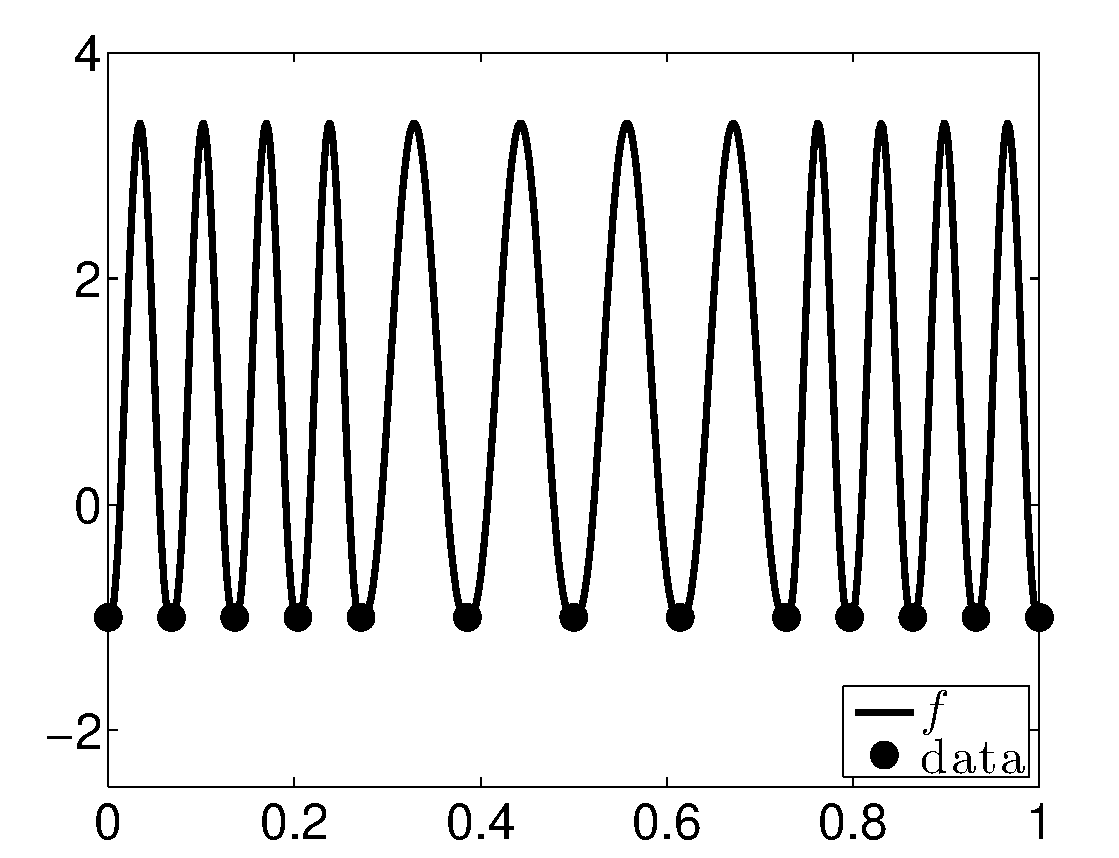
\includegraphics[width=5.5cm]{ExpositoryPaperSpikyquad.eps}
&
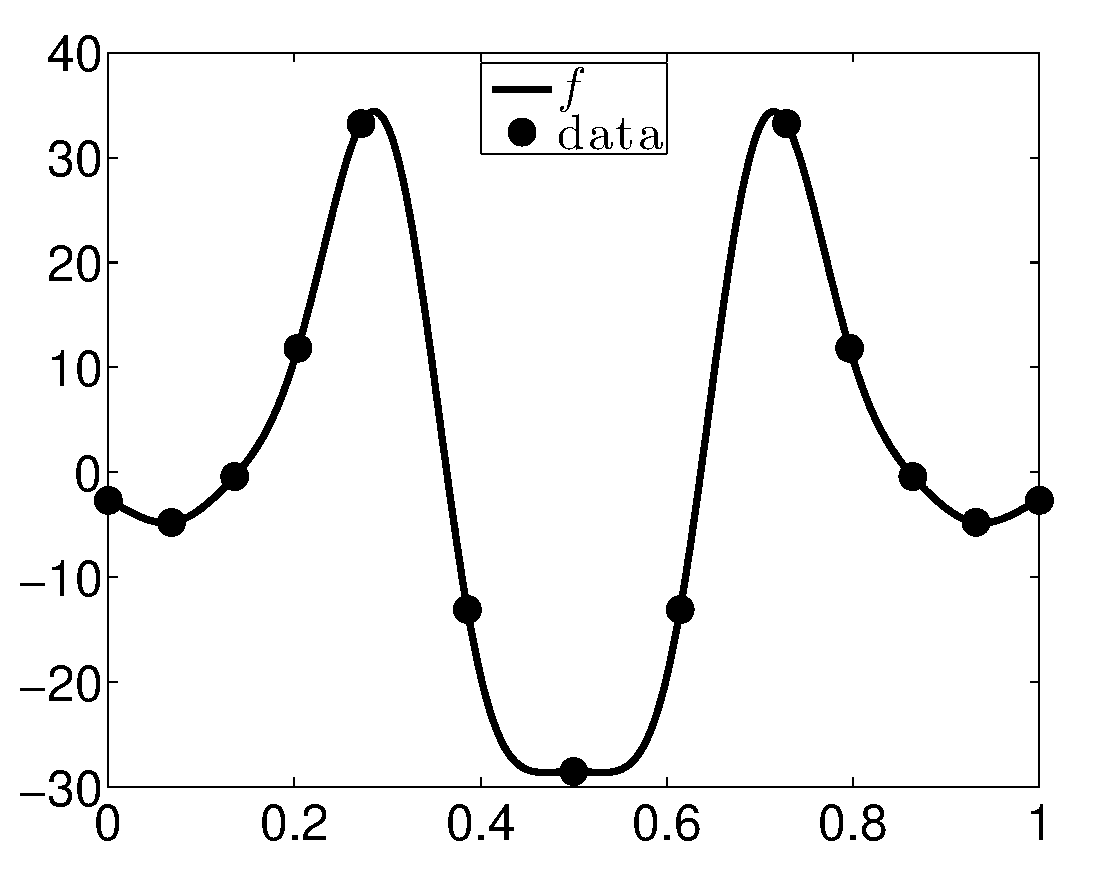
\includegraphics[width=5.5cm]{ExpositoryPaperFlukyquad.eps} \\
a) & b)
\end{tabular}
\caption{a) A spiky integrand designed to fool MATLAB's {\tt quad} and the data sampled by {\tt quad}; b) A fluky integrand designed to fool {\tt quad}. \label{fig:foolquad}}
\end{figure}

\section{A Guaranteed, Adaptive, Automatic Trapezoidal Algorithm $\integ$} \label{newalgosec}

Non-adaptive $\ballinteg$ uses no values of $f$ to determine how many trapezoids are needed to approximate the integral of $f$ because an upper bound on $\Var(f')$ is assumed.  Adaptive $\flawinteg$ uses values of $f$ to determine how how many trapezoids are needed, but in a way that might not detect a large $\Var(f')$, such as for fluky integrands.  In this section construct an adaptive algorithm that reliably estimates $\Var(f')$ for a certain cone of integrands, $\cc$.

Given any partition, $\datasites$, define an approximation to $\Var(f')$ as follows:
\begin{multline*}
\tV(f',\datasites,\{\Delta_{i}\}_{i=1}^{n-1}) : = \sum_{i=2}^{n-1} \abs{\Delta_{i} - \Delta_{i-1}}, \\
\text{where } \Delta_{i} \text{ is between } f'(x_i) \text{ and } f'(x_i^-).
\end{multline*}
Here $f'(x^-):= \lim_{\delta \downarrow 0} [f(x) - f(x-\delta)]/\delta$.  Note that $\tV$ does not involve the values of $f'$ at $x_0=a$ or $x_n=b$.  Also note that by definition
\[
\tV(f',\datasites,\{\Delta_{i}\}_{i=1}^{n-1}) \le \Var(f') \qquad \forall f \in \cv, \ \datasites, \{\Delta_{i}\}_{i=1}^{n-1}, \ n \in \naturals.
\]
The cone of integrands that our algorithm will be guaranteed to work for is defined as those functions for which $\tV(f',\datasites,\{\Delta_{i}\}_{i=1}^{n-1})$ does not underestimate $\Var(f')$ by too much:
\begin{multline} \label{conedef}
\cc := \{ f \in \cv : \Var(f') \le \fC(h) \tV(f',\datasites,\{\Delta_{i}\}_{i=1}^{n-1}) \text{ for all choices of } \\
n \in \naturals, \ \{\Delta_{i}\}_{i=1}^{n-1}, \text{ and }\datasites \text{ with } \size(\datasites) < \fh \}.
\end{multline}
Here $\fh \in (0, b-a]$ is a cut-off value, and the inflation factor $\fC:[0,\fh) \to [1,\infty)$ is a non-decreasing function.

The cone $\cc$ is defined to rule out sufficiently spiky functions because $f'$ may change much over a small distance if $f \in \cc$.  For example, if a function looks like a line on a sufficiently fine mesh, i.e., if $f'(x_i)=f'(x_i^-)=\beta$ for $i=1, \ldots, n-1$ for some real $\beta$ and some $\datasites$ with $\size(\datasites) \le \fh$, then $f$ must be the linear function $f(x)= f(a) + \beta(x-a)$.  While the triangular peak function $\tri(\cdot;t,h)$ lies inside $\cc$ for $h \ge \fh$, it lies outside $\cc$ for $h < \fh/2$.

The definition of $\cc$ does not rule out all functions with narrow spikes.  Consider the double peaked function defined as
\begin{subequations} \label{twopkdef}
\begin{gather}
\twopk(x;t,h,\pm):= \tri(x,0,\fh) \pm b\tri(x,t,h) \\
\end{gather}
\end{subequations}

Let $A$ denote the linear spline approximation using $n+1$ ordered points including the endpoints, i.e., 
\begin{multline}
\label{Andef}
A(f,\datasites)(x) \\
= \begin{cases}  \displaystyle f(x_0)\frac{x_1-x}{x_1-x_0} + f(x_1)\frac{x-x_0}{x_1-x_0}, & a=x_0 \le x < x_1, \\
\displaystyle f(x_1)\frac{x_2-x}{x_2-x_1} + f(x_2)\frac{x-x_1}{x_2-x_1}, & x_1 \le x < x_2, \\
\qquad \qquad \qquad \qquad \vdots & \qquad \quad \vdots \\
\displaystyle f(x_{n-1})\frac{x_n-x}{x_n-x_{n-1}} + f(x_n)\frac{x-x_{n-1}}{x_n-x_{n-1}}, & x_{n-1} \le x \le x_n=b.
\end{cases}
\end{multline}   
When the $x_i$ are equally spaced, i.e., $x_i=a+(b-a)i/n$, then we write $A_n(f):=A(f,\datasites)(x)$.  The composite trapezoidal rule is the integral of the linear spline based on using equally spaced data sites, i.e., $T_n(f,a,b) = \int_0^1 A_n(f)(x) \, \dif x$.  

To estimate $\Var(f')$ appearing in the theoretical error bound for the trapezoidal rule, \eqref{???}, we replace $f'$ by the derivative of the linear spline, namely, 
\begin{align*}
F(f,\datasites) &: = \Var(A(f,\datasites)') \\
& = \sum_{i=1}^{n-1} \abs{ \frac{f(x_{i+1})-f(x_{i})}{x_{i+1}-x_{i}} - \frac{f(x_i)-f(x_{i-1})}{x_i-x_{i-1}}}.
\end{align*}
When the $x_i$ are equally spaced, we use the notation $F_n(f)$.  These $F(f,\datasites)$ never overestimate $\Var(f')$.  To prove this, let $\Delta_i$ and $x_{i,\pm}$ for $i=1, \ldots, n$ satisfy
\begin{equation*}
\Delta_i:= \frac{f(x_i)-f(x_{i-1})}{x_i-x_{i-1}}, \qquad f'(x_{i,-}) \le \Delta_i \le f'(x_{i,+})/
\end{equation*}
If $f'$ is continuous, then one may take $x_{i,-}=x_{i,+}$.  Also for each $i$ let $\xi_{i,\pm}$ correspond to $x_{i,\pm}$ but with the ordering $\xi_{i,-} \le \xi_{i,+} $.  It then follows that
\begin{align*}
\Var(f') & \ge \abs{f'(\xi_{1,+}) - f'(\xi_{1,-})}  \\
& \qquad \qquad  + \sum_{i=2}^n \bigl [ \abs{f'(\xi_{i,-}) - f'(\xi_{i-1,+})}+ \abs{f'(\xi_{i,+}) - f'(\xi_{i,-})} \bigr ] \\
& = \abs{f'(\xi_{1,+}) - \Delta_1} + \abs{\Delta_1- f'(\xi_{1,-})}  \\
& \quad  + \sum_{i=2}^n \bigl[ \abs{f'(\xi_{i,-}) - f'(\xi_{i-1,+})}+ \abs{f'(\xi_{i,+}) -\Delta_i} + \abs{\Delta_i- f'(\xi_{i,-})} \bigr] \\
& =  \abs{\Delta_1- f'(\xi_{1,-})} + \abs{f'(\xi_{n,+}) - \Delta_n} \\
& \quad  + \sum_{i=2}^n \bigl[\abs{f'(\xi_{i-1,+}) -\Delta_{i-1}} + \abs{f'(\xi_{i,-}) - f'(\xi_{i-1,+})}+  \abs{\Delta_i- f'(\xi_{i,-})} \bigr] \\
& \ge \sum_{i=2}^n \abs{\Delta_i -\Delta_{i-1}} = F(f,\datasites).
\end{align*}

The cone of integrands that are not too spiky is defined to comprise those functions for which $F(f,\datasites)$ does not underestimate $\Var(f)$ by much provided that the data sites are not too far apart.  Define the mesh size of a set of data sites as the maximum width between adjacent  sites:
\[
h(\datasites):=\max_{1 \le i \le n} x_i-x_{i-1}.
\]
The cone of integrands for which our new adaptive algorithm $\integ$ will succeed is 
\begin{multline}
\cc:=\biggl \{f \in \cv : \Var(f') \le \fC(\size(\datasites)) F(f,\datasites)  \\
\text{ for all partitions } \datasites \text{ of } [a,b] \text{ with } h(\datasites) < \fh \biggr \}.
\end{multline}

There are two parameters defining this cone, an inflation factor $\fC \ge 1$ and positive key mesh size, $\fh$.  The inverse of the inflation factor, $\fC^{-1}$, represents the factor that $F(f,\datasites)$ is allowed to underestimate $\Var(f')$ by in the limit of vanishing $h(\datasites)$.  

Functions whose first derivative has zero total variation are lines.  Analogously, any function $f$ satisfying $F(f,\datasites)=0$ resembles a line when sampled at $\datasites$.  The role of $\fh$ can be understood by noting that if $f\in \cc_{\fC,\fh}$ resembles a line when sampled over data sites with mesh size less than $\fh$, then $f$ must indeed be a line because by the definition of $\cc_{\fC,\fh}$ we know that $\Var(f')=0$. Another way to understand $\fh$ is that $\cc_{\fC,\fh}$ contains no functions with significant spikes narrower than $\fh$ because the sampling scheme might not detect them.

Our composite trapezoidal 

\begin{algo}\label{adaptintegalgo} [$\integ$, Adaptive, for Cones $\cc_{\fC,\fh}$] Given an interval, $[a,b]$, an inflation factor, $\fC>1$, a positive key mesh size, $\fh$, a positive error tolerance, $\varepsilon$, and a routine for generating values of the integrand, $f$, set $j=1$ and $n_1 = \left \lfloor (b-a)/\fh \right \rfloor +1$.
\begin{description}
\item[Step 1] Compute the error estimate $\terr(f,n_j)$ according to \eqref{guarerr}.

\item [Step 2] If $\terr(f,n_j) \le \varepsilon$, then return the trapezoidal rule approximation $T_{n_j}(f)$ as the answer.  

\item [Step 3] Otherwise let $n_{j+1}=2 n_j$, increase $j$ by one, and go to Step 1.

\end{description}
\begin{equation}\label{algo1n}
n = \Bigg \lceil (b-a)\sqrt{\frac{\sigma}{8\varepsilon}} \Bigg \rceil,
\end{equation}
and return the trapezoidal rule $\ballinteg(f,a,b,\varepsilon)=T_n(f,a,b)$ as the answer.
\end{algo}
Using this definition of linear spline we focus on the semi-norm defined by $f \mapsto \Var(f-A_1(f))$.  Like $f \mapsto \Var(f')$ this weaker semi-norm also vanishes for functions that are linear in $x$.  If $\Var(f')$ is finite, then it follows that $\Var(f) = \norm[1]{f'}:=\int_0^1 \abs{f(x)} \, \dif x$, so the weaker semi-norm may be written as $f \mapsto \norm[1]{f'-f(1)+f(0)}$.  It is shown in \ocite{HicEtal14b}*{Section 5.1} that 
\begin{equation} \label{weaknorm}
2 \norm[1]{f'-f(1)+f(0)} \le \Var(f') \qquad \forall f \text{ with } \Var(f')<\infty.
\end{equation}

The data-driven quantity 
\begin{equation} \label{weaknormalgo}
\norm[1]{A_n(f)'-f(1)+f(0)}= \sum_{i=1}^n \abs{f\left(\frac in \right)-f\left(\frac{i-1}n \right) - \frac{f(1)-f(0)}{n}}
\end{equation}
always underestimates $\norm[1]{f'-f(1)+f(0)}$, but not by much provided that $\Var(f')$ is not too large. Again in \ocite{HicEtal14b}*{Section 5.1} it is shown that 
\begin{equation} \label{errweaknorm}
0 \le \norm[1]{f'-f(1)+f(0)} - \norm[1]{A_n(f)'-f(1)+f(0)} \le \frac{\Var(f')}{2n}.
\end{equation}

At this point it seems that we have reached a dead end because we have an error bound in terms of $\Var(f')$, just like the trapezoidal rule error bound \eqref{traperrbd}.  However, we make a further assumption that $f$ lies in the cone defined as 
\begin{equation} \label{conedef}
\cc_{\tau} := \{f : \Var(f') \le \tau \norm[1]{f'-f(1)+f(0)} \}.
\end{equation}
This cone consists of functions whose stronger semi-norms are not too much greater than their weaker semi-norms.  The set $\cc_{\tau}$ is called a cone because $f \in \cc_{\tau}$ implies that $cf \in \cc_{\tau}$ for all $c \in \reals$.  Substituting this upper bound on $\Var(f')$ into \eqref{errweaknorm} and re-arranging the terms implies a data-driven upper bound on  $\Var(f')$:
\begin{multline} \label{varfprimeless}
\Var(f') \le \tau \norm[1]{f'-f(1)+f(0)}  \\
\le \frac{\tau \norm[1]{A_n(f)'-f(1)+f(0)}}{1-\tau/(2n)} \qquad \forall f \in \cc_{\tau},
\end{multline}
provided that $n>\tau/2$.  There is also a companion bound in the other direction based on \eqref{weaknorm} and \eqref{errweaknorm}:
\begin{equation} \label{varfprimegreat}
\norm[1]{A_n(f)'-f(1)+f(0)} \le \norm[1]{f'-f(1)+f(0)} \le \frac{\Var(f')}{2}.
\end{equation}

Plugging \eqref{varfprimeless} into \eqref{traperrbd} yields the following guaranteed error bound for the trapezoidal rule:
\begin{equation} \label{guarerr}
\err(f,n) \le \terr(f,n) := \frac{\tau \norm[1]{A_n(f)'-f(1)+f(0)}} {4n(2n-\tau)} \qquad \forall f \in \cc_{\tau}.
\end{equation}
This new error bound can then be used to construct the following adaptive, automatic quadrature algorithm, which is a simplification of \ocite{HicEtal14b}*{Algorithm 4}:

\begin{algo}[Adaptive, Automatic, for Cones] \label{conealgo} Given $\tau>0$, and an error tolerance, $\varepsilon$, let $j=1$ and $n_1=\lceil (\tau+1)/2 \rceil$.

\begin{description} 

\item[Step 1] Compute the error estimate $\terr(f,n_j)$ according to \eqref{guarerr}.

\item [Step 2] If $\terr(f,n_j) \le \varepsilon$, then return the trapezoidal rule approximation $T_{n_j}(f)$ as the answer.  

\item [Step 3] Otherwise let $n_{j+1}=2 n_j$, increase $j$ by one, and go to Step 1.

\end{description}
\end{algo}

Error bound \eqref{guarerr} is used to prove that Algorithm \ref{conealgo} is successful for integrands in $\cc_{\tau}$.  Let $N(f,\varepsilon,\tau)$ denote the eventual number of trapezoids required by this algorithm.  Because the algorithm is adaptive, the number of trapezoids depends on the particulars of $f$ as well as the error tolerance.  The two bounds \eqref{varfprimeless} and \eqref{varfprimegreat} may be used to derive both lower and upper bounds on $N(f,\varepsilon,\tau)$:

\begin{theorem}\cite{HicEtal14b}*{Theorem 7} \label{conealgothm}
Let $N(f,\varepsilon,\tau)$ denote the final $n_j$ in Algorithm \ref{conealgo}.  Then this algorithm is successful for all functions in $\cc_{\tau}$,  i.e.,  $\abs{\int_0^1 f(x) \, \dif x - T_{N(f,\varepsilon,\tau)}(f)} \le \varepsilon$.  Moreover, $N(f,\varepsilon,\tau)$ is bounded below and above as follows:
\begin{multline}
\max \left(\left \lceil\frac{\tau+1}{2} \right \rceil, \left \lceil \sqrt{\frac{ \Var(f')}{8\varepsilon}} \right \rceil \right) \\
\le \max \left(\left \lceil\frac{\tau+1}{2} \right \rceil, \left \lceil \sqrt{\frac{\tau \norm[1]{f'-f(1)+f(0)}}{8\varepsilon}} \right \rceil \right) \\
\le
N(f,\varepsilon,\tau) \\
\le \sqrt{\frac{\tau \norm[1]{f'-f(1)+f(0)}}{2\varepsilon}} + \tau + 3
\le \sqrt{\frac{\tau \Var(f') }{4\varepsilon}} + \tau + 3.
\end{multline}
\end{theorem}

Note that the cost of the algorithm depends on $\Var(f')$, but without the algorithm needing to know $\Var(f')$ in advance.   Comparing the two error bounds on which Algorithms \ref{ballalgo} and \ref{conealgo} are based and applying the , we note that 
\begin{equation*}
\frac{\Var(f')}{\sigma} \le
\frac{\terr(f,n)}{\oerr(f,n)}
\le \frac{\tau\Var(f')}{\sigma (2-\tau/n)}.
\end{equation*}



For an integrand like \eqref{GaussExample} where $\Var(f')$ is known, the number of trapezoids required by Algorithm \ref{conealgo} is no greater than  $\sqrt{\tau \Var(f') /(4\varepsilon)} + \tau + 3$, whereas for Algorithm \ref{ballalgo} with $\sigma=\Var(f')$ the number of trapezoids is no more than $\bigl \lceil \sqrt{\Var(f') /(8\varepsilon)} \, \bigr\rceil$.  The extra cost for Algorithm \ref{conealgo} comes in the form of the factor $\sqrt{2\tau}$ and the additional additive term of $\tau+1$.  On the other hand, if $\Var(f')$ is not known in advance, then the disadvantage of Algorithm  \ref{ballalgo} is that if $\Var(f')$ is not known in advance, and $\sigma$ is chosen conservatively, then Algorithm \ref{conealgo} could cost arbitrarily more than $\sqrt{\Var(f') /(8\varepsilon)}+1$ in the limit of , 

\section{Discussion} \label{discusssec}

\section{Acknowledgements}  The authors are grateful for discussions with a number of colleagues. This research is supported in part by grant NSF-DMS-1115392.

\bibliography{FJH22,FJHown23}
\end{document}

The Bernoulli polynomials are described by \ocite{AbrSte64}*{Chap.\ 23, \url{http://dlmf.nist.gov/24}}.  The first six are defined as follows 
\begin{subequations} \label{Bernoulli}
\begin{gather} 
B_0(x) = 1, \qquad B_1(x) = x-1/2,  \qquad 
B_2(x)=1/6 - x(1-x), \\ 
B_3(x) = \frac{1}{2} x(1-x)(1-2x), \qquad B_4(x) = -1/30 + [x(1-x)]^2, \\
B_5(x) = \frac{1}{6} x(1-x)(1-2x)(1 + 3 x - 3 x^2).
\end{gather}
\end{subequations}

\subsection{Necessary Conditions for Failure of the Error Estimate} 
Integrands that satisfy \eqref{failcond} and fool the error estimate in \eqref{baderr} must satisfy certain conditions.  First note that the error bound in \eqref{traperrbd} implies that
\[
\Var(f') \ge 8n^2 \err(f,n) =  16n^2 \asymp n^2 \qquad \text{as } n \to \infty,
\]
so the total variation of the first derivative must be increasingly large as the number of trapezoids increases.  Moreover, the trapezoidal rule added to the error estimate in \eqref{baderr} is actually Simpson's rule:
\begin{align*}
S_n(f) &:= T_n(f) + \herr(f,n) = \frac{4T_n(f) - T_{n/2}(f)}{3} \\
& = \frac{1}{3n} \left [ f(0) + 4 f(1/n) + 2 f(2/n) + 4 f(3/n) + \cdots + 4 f(1-1/n) + f(1) \right].
\end{align*}
The error bound of Simpson's rule then serves as an bound on the error of the error estimate \cite{BraPet11a}*{Sect.\ 7.3, p.\ 231}:
\begin{equation} \label{Simperrbd}
\abs{\err(f,n) - \herr(f,n)} = \abs{\int_0^1 f(x) \, \dif x - S_n(f)} \le \frac{\Var(f''')}{36n^4}, \qquad \frac{n}2 \in \naturals. 
\end{equation}
So, integrands satisfying \eqref{failcond} must also satisfy
\[
\Var(f''') \ge 36n^4 \abs{\err(f,n) - \herr(f,n)} =  36n^4 \asymp n^4 \qquad \text{as } n \to \infty.
\]
Thus, the total variation of the third derivative must increase even faster than the minimum increase of $\Var(f')$ as the number of trapezoids increases.

The derivatives of Bernoulli polynomials are multiples of lower degree Bernoulli polynomials and the integrals of nonconstant Bernoulli polynomials vanish (see \ocite{AbrSte64}*{Chap.\ 23, \url{http://dlmf.nist.gov/24}}):
\[
B'_n(x) = n B_{n-1}(x), \quad \int_0^1 B_{n+1}(x) \, \dif x, \qquad n \in \naturals.
\]
The formula for the derivatives facilitates the computation of the total variation of the spiky and fluky examples above, confirming that the variations of their first and third derivatives satisfy the above inequalities.  For the spiky integrand defined in \eqref{spiky},
\begin{subequations} \label{spikyvariation}
\begin{gather}
%f'_{\text{spiky}}(x;n) = 240 n B_3(\bbl nx \bbr), \qquad f''_{\text{spiky}}(x;n) = 720 n^2 B_2(\bbl nx \bbr), \\ f'''_{\text{spiky}}(x;n) = 1440 n^3 B_1(\bbl nx \bbr), \\
\Var(f_{\text{spiky}}(\cdot;n))= \frac{15n}{2}, \qquad  \Var(f'_{\text{spiky}}(\cdot;n))= \frac{80n^2}{\sqrt{3}} > 16 n^2, \\
\Var(f''_{\text{spiky}}(\cdot;n))= 360n^3, \qquad \Var(f'''_{\text{spiky}}(\cdot;n))= 1440n^4 > 36n^4.
\end{gather}
\end{subequations} 
For the fluky integrand defined in \eqref{fluky},
\begin{subequations} \label{spikyvariation}
\begin{gather}
%f'_{\text{fluky}}(x;n) = - 30 n^2 [B_1(x) + 2 n^2 B_3(x)], \\ f''_{\text{fluky}}(x;n) = -30 n^2 [1 + 6 n^2 B_2(x)], \qquad f'''_{\text{fluky}}(x;n) = -360 n^4 B_1(x), \\
\Var(f_{\text{fluky}}(\cdot;n))= \frac{15}{8} (8 - 4 n^2 + n^4),  \\
\Var(f'_{\text{fluky}}(\cdot;n))= \frac{10 n}{3}  \Bigl[9 n + 2 \sqrt{3(-2 + n^2)^3} \Bigr ]  > 16 n^2, \\
\Var(f''_{\text{fluky}}(\cdot;n))= 90n^4, \qquad \Var(f'''_{\text{fluky}}(\cdot;n))= 360n^4 > 36n^4.
\end{gather}
\end{subequations}  

For the spiky integrand the asymptotic order of the total variation for large $n$ increases with the order of the derivative while for the fluky integrand it stays the same.  Specifically,
\[
\Var(f^{(j)}_{\text{spiky}}(\cdot;n)) \asymp n^{j+1}, \quad \Var(f^{(j)}_{\text{fluky}}(\cdot;n)) \asymp n^{4}, \qquad j=0, \ldots, 3.
\]
This difference in asymptotic behaviors distinguishes whether a better error bound developed in the next section will be successful:  no for the spiky integrand , but yes for the fluky integrand.


\iffalse 
\subsection{When \texttt{cos} Fails}

Before addressing the more difficult problem of numerical integration, let's consider the simpler problem of producing values of $\cos(x)$ on a computer or calculator with a double precision number system.  Double precision means that calculations are done using about $15$ decimal digits of accuracy, so we expect \texttt{cos($x$)}\footnote{We use the teletype font to denote a numerical algorithm here and elsewhere in this article.} on a computer to satisfy
\begin{equation} \label{coserrexpect}
\abs{\cos(x)-\texttt{cos($x$)}} \le 10^{-15}.
\end{equation}

The numerical calculation \texttt{cos($x$)} first identifies $y=x+n\pi$ near zero, where $n$ is an integer. Noting that $\cos(x)=(-1)^n\cos(y)$, the algorithm approximates $\cos(y)$ by a high degree polynomial or rational function.  This approach achieves the desired accuracy in many cases, but \texttt{cos($x$)} has poor accuracy for very large $x$.  For example, in MATLAB one obtains
\begin{alltt}
>> cos(1e17*pi)
ans =
    -5.300447339957113e-01
\end{alltt}
whereas one might hope for an answer of $1$\footnote{While our numerical examples in this article are coded in MATLAB \cite{MAT8.1}, the principles illustrated apply universally to numerical algorithms implemented in other programming languages or software packages.}.   The reason for the large error here is that the computer number system with $15$ decimal digits cannot distinguish between $10^{17}\pi$ and $(10^{17}+1)\pi$, whose cosine values are quite different. 

This example illustrates that virtually all numerical algorithms can be inaccurate.  The user should know for what inputs an algorithm might not give the desired accuracy.  For the \texttt{cos} algorithm, \eqref{coserrexpect} is wrong and should be replaced by 
\[
\abs{\cos(x)-\texttt{cos($x$)}} \le \min(2,10^{-15}(1+\abs{x})).
\]

\subsection{Why Numerical Integration Is Needed?}
\fi

\iffalse The problem of numerical integration is much harder than the problem of evaluating the cosine function.  For \texttt{cos($x$)} the input $x$ is a number, which is known to $15$ significant digits.  For integration the key input is an imperfectly known function.  
\fi
